\documentclass{article}
\usepackage[utf8]{inputenc}
\usepackage[margin=1in]{geometry}

\usepackage{algorithm}
\usepackage[noend]{algpseudocode}
\algnewcommand\Or{\textbf{ or }}
\algnewcommand\Init{\textbf{initialize }}
\MakeRobust{\Call}

\title{Lowest Common Ancestor}
\author{Daniel Wisdom}
\date{December 1 2017}

\usepackage{float}
\usepackage{tikz}
\usetikzlibrary{calc,shapes.multipart,chains,arrows,positioning}

\definecolor{myseagreen}{RGB}{230,250,250}
\tikzstyle{vertex}=[draw,fill=myseagreen,circle,minimum size=24pt,inner sep=0pt]

\begin{document}

\maketitle

\section{Introduction}
If we are given an undirected graph $G$ that contains no cycles, then we may designate any one of its vertices as the root. By rooting the tree, we give all of the edges the natural direction of pointing towards the root. Additionally, we can define the height of a vertex as its distance to the root. The LCA, or Lowest Common Ancestor, problem involves finding the node of maximum height that is an ancestor of two given nodes.  

\begin{figure}[H]
\centering
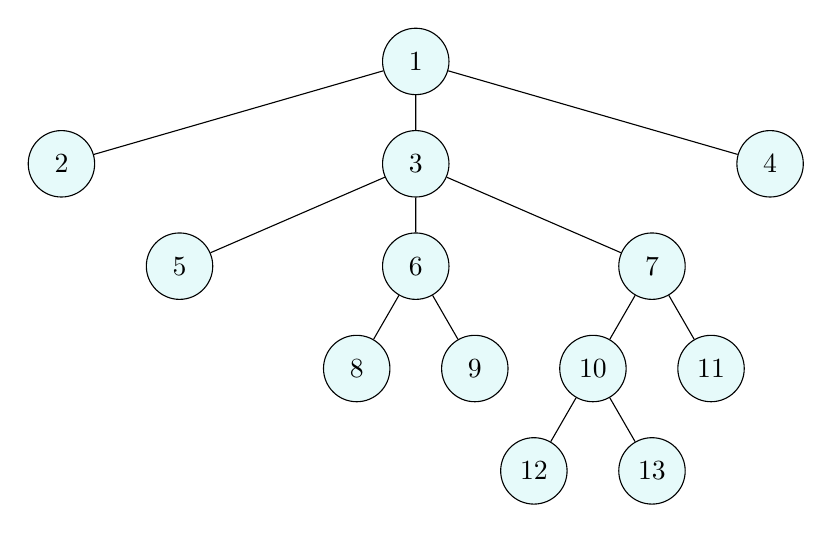
\begin{tikzpicture}[level/.style={sibling distance=15mm,level distance=13mm}]
\node [vertex] {1}
  child [sibling distance=45mm] {
    node [vertex] {2}
  }
  child [sibling distance=45mm] {
    node [vertex] {3}
    child [sibling distance=30mm] { 
        node [vertex] {5} 
    }
    child [sibling distance=30mm]{
      node [vertex] {6}
      child { node [vertex] {8} }
      child { node [vertex] {9} }
    }
    child [sibling distance=30mm] {
      node [vertex] {7}
      child {
        node [vertex] {10}
        child { node [vertex] {12} }
        child { node [vertex] {13} }
      }
      child { 
        node [vertex] {11} 
      }
    }
  }
  child [sibling distance=45mm] {
    node [vertex] {4}
  };
\end{tikzpicture}
\end{figure}


\section{DFS}

Before we begin finding the LCA, it is in our best interest to be able to calculate the height of each node (for reasons that will become apparent later). To do this, we can simply do a DFS starting at the root. This has complexity $O(N)$. We will use $h(u)$ for the height of node $u$.


\section {Naive Solution}

Supposed we want to find the LCA of nodes $u$ and $v$ such that $h(u)>h(v)$. Notice that the LCA cannot be any node with height greater than $h(v)$, so we repeatedly reassign $u$ with its parent until $u$ and $v$ have the same height. Now, we repeatedly reassign both $u$ and $v$ to their parents until they point to the same node. This node is the LCA of $u$ and $v$. This algorithm is equivalent to moving $u$ and $v$ one level up at a time until they match.

Note that this has worst case time complexity $O(N)$. This occurs when the tree is effectively a linked list. Additionally, this algorithm requires $O(N)$ preprocessing because we must calculate the heights of each node. Unfortunately, many problems will require us to perform multiple LCA queries, so $O(N)$ is too slow. 


\section {$2^n$ Jump Pointers}

Based on the previous two solutions, we would now like to develop an algorithm that balances both preprocessing and query time. Consider the $N \times \log N$ table $A$, where $A(i, j)$ represents the node that is $2^j$ steps above node $i$. We can compute the contents of the table with the following dynamic programming formulation: 
$$A(i, 0) = parent(i)$$
$$A(i, j+1) = A( A(i, j), j )$$

\noindent The recurrence relation is analogous to first moving $2^j$ steps to node $A(i, j)$, and then moving an additional $2^j$ steps to traverse a total of $2^{j+1}$ steps above $i$. Thus, $A$ can be computed in $O(N \log N)$. 

Now, to actually find the LCA of $u$ and $v$, we employ a similar approach taken in the first Naive Solution, but using our $2^n$ jump pointer table. Assume $h(u) > h(v)$ and let $d = h(u) - h(v)$ be the difference in height. Note that $d$ can be written as a sum of at most $\log d$ unique powers of 2 (Hint: consider the binary representation of $d$). Since $A$ tells us how to move nodes upwards in increments of powers of two, this means that $u$ can be moved $d$ steps upwards by making $\log d$ lookups in $A$. Once $u$ and $v$ are at the same height, we repeatedly move them upwards by the largest power of 2 such that $u$ and $v$ do not point to the same node. This works because if $A(u, i) \neq A(v, i)$, then $LCA(u, v) = LCA(A(u, i), A(v, i))$. In this manner, we can repeatedly reduce the distance from $u$ and $v$ to $LCA(u, v)$ by a factor of at least two.  Thus, this takes $O(\log N)$ lookups in $A$, so the complexity of each LCA query is $O(\log N)$. 

\section{Another View of LCA}

Here I will present another $O(\log N)$ solution to LCA which you may find easier to code.  Along the path from node $u$ to $v$ the node with minimum height must be the LCA of $u$ and $v$.  This means LCA($u$,$v$) can be found by a range min query of the path from $u$ to $v$.

Now we will do a traversal of the graph.  This traversal will create two things: a list of heights and a mapping of each node to the first index at which it appears in the list.

\begin{algorithm}[H]
\caption{Traversal}
\begin{algorithmic}
\Function{traverse}{node $u$}
    \State index[u] = current list size
    \State Append $h(u)$ to the list
    \For {each child $v$ of $u$}
        \State traverse($v$)
        \State Append $h(u)$ to the list
    \EndFor
\EndFunction
\end{algorithmic}
\end{algorithm}

The traversal will always produce a list of $2N-1$ elements, so we can allocate an array in the beginning and avoid dynamic arrays.

The important property of this traversal is that for every pair of nodes $u$ and $v$, LCA($u$,$v$) will appear at least once in the list between any two occurrences of $u$ and $v$.  There will be nodes listed between $u$ and $v$ which are not on the path from $u$ to $v$, but they will always have a larger height than the LCA.  This means a range min query from an occurrence of $u$ to an occurrence of $v$ will find the LCA($u$,$v$).  Range min queries can be answered by Segment Trees in $O(N\log N)$ preprocessing and $O(\log N)$ query time.

%find me more problems pls
\section {Problems}

\begin{enumerate}
    \item USACO December 2015, Platinum Contest Problem 1, Max Flow
    
    Farmer John has installed a new system of N-1 pipes to transport milk between the N stalls in his barn $(2\leq N\leq 50,000)$, conveniently numbered 1…N. Each pipe connects a pair of stalls, and all stalls are connected to each-other via paths of pipes.
FJ is pumping milk between K pairs of stalls $(1\leq K\leq 100,000)$. For the ith such pair, you are told two stalls $s_i$ and $t_i$, endpoints of a path along which milk is being pumped at a unit rate. FJ is concerned that some stalls might end up overwhelmed with all the milk being pumped through them, since a stall can serve as a waypoint along many of the K paths along which milk is being pumped. Please help him determine the maximum amount of milk being pumped through any stall. If milk is being pumped along a path from $s_i$ to $t_i$, then it counts as being pumped through the endpoint stalls $s_i$ and $t_i$, as well as through every stall along the path between them.
    \item Codeforces 702E Analysis of Paths in Functional Graph
    
    You are given a directed graph of $N$ nodes.  Every node has exactly one edge leaving it, with a specified weight.  There may be cycles in the graph.  There is exactly one path of length $(1\leq k\leq 100,000)$ from every node.  For the length $k$ path from node $i$, quickly find the sum and minimum edge weight along the path.  

\end{enumerate}

\end{document}
